% =============================================================================
% FAECO 中文期刊版式（计算机辅助设计与图形学学报模板近似）
% 字体说明：模板要求方正书宋_GBK/方正仿宋_GBK/黑体/Times New Roman。
% 方正 GBK 字库为商业字体，需作者自行购买安装；当前以系统宋体/黑体/仿宋近似。
% 安装方正字库后，将下方 FZ 字体变量替换为对应方正字体名即可。
% =============================================================================
\documentclass[twocolumn,10pt,fontset=windows]{ctexart}

% -----------------------------------------------------------------------------
% 字体（方正 GBK 安装后替换此处）
%   正文:    \setCJKmainfont{方正书宋_GBK}
%   标题:    \setCJKsansfont{方正黑体_GBK}
%   仿宋:    \setCJKfamilyfont{fzfs}{方正仿宋_GBK}
% 当前用系统字体近似（fontset=windows: 宋体/黑体/楷体/仿宋）
% -----------------------------------------------------------------------------
\setmainfont[Path=./fonts/,Extension=.ttf,UprightFont=times,BoldFont=timesbd,ItalicFont=timesi,BoldItalicFont=timesbi]{Times New Roman}
\setCJKmainfont[Path=./fonts/,Extension=.ttf]{FZShuSong-Z01}
\setCJKsansfont[Path=./fonts/,Extension=.ttf]{SimHei}
\newCJKfontfamily\songfamily[Path=./fonts/,Extension=.ttf]{FZShuSong-Z01}
\newCJKfontfamily\fangfamily[Path=./fonts/,Extension=.ttf]{FZFangSong-Z02}
\newCJKfontfamily\heifamily[Path=./fonts/,Extension=.ttf]{SimHei}
\usepackage{amsmath,amssymb}
\usepackage{newtxmath}
\let\songti\songfamily\let\heiti\heifamily\let\fangsong\fangfamily
\usepackage{booktabs}
\usepackage{graphicx}
\usepackage{subfig}
\usepackage{float}
\usepackage{array}
\usepackage[nocompress]{cite}
\usepackage[hidelinks]{hyperref}
\usepackage{xurl}
\usepackage{algorithm}
\usepackage{algpseudocode}
\usepackage{multirow}
\usepackage{geometry}
\usepackage{placeins}
\usepackage{dblfloatfix}

% 版面：A4 双栏，栏宽 21.59 字符、栏间距 3 字符（以 3zw 近似）
\geometry{a4paper,left=2.0cm,right=2.0cm,top=2.1cm,bottom=2.1cm,columnsep=31.5pt}

\renewcommand{\eqref}[1]{\textup{（\ref{#1}）}}
\graphicspath{{../figures/}}
\setlength{\emergencystretch}{3em}
\Urlmuskip=0mu plus 3mu\relax
\raggedbottom
\setlength{\floatsep}{6pt plus 2pt minus 2pt}
\setlength{\textfloatsep}{8pt plus 2pt minus 2pt}
\setlength{\intextsep}{6pt plus 2pt minus 2pt}
\setlength{\dblfloatsep}{6pt plus 2pt minus 2pt}
\setlength{\dbltextfloatsep}{8pt plus 2pt minus 2pt}

% -----------------------------------------------------------------------------
% 标题层级（模板：1级11.5pt黑体 / 2级五号黑体 / 3级10pt书宋）
% -----------------------------------------------------------------------------
\ctexset{
  section = {format=\heiti\fontsize{11.5}{15}\selectfont, beforeskip=6pt, afterskip=4pt},
  subsection = {format=\heiti\fontsize{10.5}{14}\selectfont, beforeskip=5pt, afterskip=3pt},
  subsubsection = {format=\songti\fontsize{10}{13}\selectfont, beforeskip=4pt, afterskip=2pt}
}

% 图题（书宋9pt）、表题（黑体9pt）、表注/分图题（书宋8pt）
\usepackage{caption}
\DeclareCaptionFont{songti}{\songti}
\DeclareCaptionFont{heiti}{\heiti}
\captionsetup[figure]{font={songti,small},labelfont={bf},skip=3pt}
\captionsetup[table]{font={heiti,small},labelfont={bf},skip=3pt}
% subfig is not used in this manuscript; do not configure an unused subfloat caption.
\captionsetup{labelsep=space}

\begin{document}

\pagestyle{plain}

% -----------------------------------------------------------------------------
% 中文首部：标题/作者/单位/摘要/关键词/中图法分类号/DOI
\twocolumn[
\vspace*{-0.25cm}
\begin{center}
{\heiti\zihao{3} FAECO：面向预布局门级时序 ECO 的失效驱动候选搜索}\par
\vspace{6pt}
{\fangsong\zihao{4} 佟亚龙}\par
\vspace{4pt}
{\songti\fontsize{8}{12}\selectfont（国防科技大学计算机学院，长沙 410073）}\par\vspace{2pt}
{\songti\fontsize{8}{12}\selectfont E-mail：tyl2003@nudt.edu.cn（通信作者）}\par
\vspace{6pt}
\end{center}
\begin{flushleft}
  {\heiti\fontsize{8.5}{13}\selectfont 摘\quad 要：}{\songti\fontsize{8.5}{13}\selectfont 针对预布局门级时序 ECO 中缓冲器插入和门尺寸调整难以压缩深层逻辑的问题，本文提出失效驱动候选搜索引擎（Failure-Aware ECO，FAECO）。该方法在已映射网表的违例扇入锥上构造多特征加权割，将局部功能保持候选的可用性、关键路径覆盖和候选规模编码为割权重，并根据候选失败类型更新后续搜索。候选先经库函数和结构规则筛选，再由 OpenSTA 在理想线网模式下测量时序收益；满足条件的候选进入基于标准寄生交换格式（SPEF）的简化复测。在三组测试集上，FAECO 分别实现 8/8、18/19 和 2/3 个电路的严格 WNS 改善；其中 ITC-99 的其余 1 个电路与基线持平，未出现回退。混合策略平均改善 1.07 ns，真实布局布线后 5/8 个电路保持改善。FAECO 扩展了深层逻辑的时序修复空间。}
\par
\vspace{4pt}
{\heiti\fontsize{8.5}{13}\selectfont 关键词：}{\songti\fontsize{8.5}{13}\selectfont 时序 ECO；门级局部重构；多特征加权割；失效驱动反馈；简化 SPEF 门控；预布局时序优化}\par
\vspace{2pt}
{\songti\fontsize{8.5}{13}\selectfont 中图法分类号：TP391.41}\par
\vspace{2pt}
{\songti\fontsize{8.5}{13}\selectfont DOI：10.3724/SP.J.1089.2026-00001}
\end{flushleft}
\vspace{4pt}
% 英文题录
\begin{center}
{\bfseries\fontsize{13.5}{18}\selectfont FAECO: Failure-Aware Candidate Search for Pre-Placement Gate-Level Timing ECO}\par
\vspace{3pt}
{\normalsize Tong Yalong\par}
\vspace{3pt}
{\small \itshape (College of Computer Science, National University of Defense Technology, Changsha 410073, China)}\par
\vspace{4pt}
\end{center}
\begin{flushleft}
  {\bfseries Abstract:} {\small We present Failure-Aware ECO (FAECO), a failure-aware candidate-search engine for pre-placement gate-level timing ECO, to address the limited ability of buffer insertion and gate sizing to compress deep logic. FAECO constructs a multi-feature weighted cut over violating fan-in cones of mapped netlists, encoding local function-preservation availability, critical-path coverage, and candidate size, and updates the search through candidate failures; candidates are screened by library-function and structural rules, accepted by OpenSTA measurements on ideal nets, and subjected to simplified rechecking using SPEF. Across three benchmark sets, FAECO achieves strict WNS improvement on 8/8, 18/19, and 2/3 circuits, respectively; on ITC-99, the remaining circuit matches the baseline without regression. The mixed strategy achieves a mean improvement of 1.07 ns, and 5/8 circuits retain an improvement after real placement and routing. FAECO expands the timing-repair space for deep logic.}\par
\vspace{3pt}
{\bfseries Key words:} {\small gate-level timing ECO; local restructuring; multi-feature weighted cut; failure-aware feedback; simplified SPEF gate; pre-placement timing optimization}\par
\end{flushleft}
]%


% =============================================================================
% I. 引言
% =============================================================================
\section{引言}

工程变更命令（engineering change order，ECO）按修复目标可分为功能 ECO 与时序 ECO：前者修复逻辑功能错误，后者修复时序违例。本文聚焦综合后、布局布线前的门级时序 ECO。本文将“局部重构”定义为在已映射网表的违例扇入锥上执行等价单元替换、门尺寸调整、缓冲器插入和少量多门组合，完整的寄存器传输级（register-transfer level，RTL）综合属于上游网表生成阶段。传统时序 ECO 主要依赖缓冲器插入（buffer insertion，B）与门尺寸调整（gate sizing，G），通过调整单元延迟修复最差负松弛（worst negative slack，WNS）与总负松弛（total negative slack，TNS）。在严重路径违例下，B/G 优化能力不足，其结构重映射与缓冲插入变体同样受候选空间限制\cite{chen2012metal,chen2012fixability,liang2012buffer,ho2010eco}。

工业实践中，将违例锥（最差负松弛路径所在的扇入逻辑锥）整体替换为时序友好补丁的做法比 B/G 更稳定，但这类方法需要工业数据，公开工具链难以复现。由于逻辑补丁构造和物理优化彼此割裂，补丁替换常在功能等价验证与时序收益之间反复失配，导致收敛缓慢甚至失败。

上述方法留下三个需要在公开工具链上量化的问题：第一，候选构造阶段的功能保持偏好对无效候选数量的影响；第二，理想线网时序收益与线载变化之间的筛选关系；第三，候选失败信息对下一轮搜索空间的收缩作用。
\noindent\parbox{\columnwidth}{实验范围为已映射门级网表和公开的 SKY130 HD 标准单元库；分析对象为局部时序 ECO，功能保持采用构造级检查，顺序等价性和完整逻辑重综合采用独立验证流程。}

\begin{samepage}
实验对象按如下方式选取：主实验选用经典顺序电路基准集 ISCAS89\cite{iscas89}；跨测试集实验选用 ITC-99 基准电路族中能够在相同流程下成功映射到 SKY130 HD 的电路\cite{itc99}；另从开源、面向尺寸优化的 RISC-V 处理器 PicoRV32 的寄存器传输级设计中选取三个结构不同的子模块\cite{picorv32}。布局布线前的寄生复测采用标准寄生交换格式（Standard Parasitic Exchange Format，SPEF）的简化模型。
\end{samepage}

所提 FAECO 将门级候选搜索分解为三阶段流水线，在候选构造阶段同时编码局部功能保持能力与时序目标，使时序失败能够转化为下一轮搜索的反馈信号。主要贡献如下：

\begin{enumerate}
  \item \textbf{失效驱动的多特征加权割与闭环细化机制}：将局部功能保持候选的可用性、关键路径覆盖和候选规模编码为割图权重，定义六类失败（F1--F6）及其对应的下一轮搜索动作，并以简化 SPEF 进行物理筛选。
\item \textbf{跨测试集评估}：在 ISCAS89 主实验集、能够在相同流程下映射到 SKY130 HD 的 ITC-99 电路，以及 PicoRV32 的三个结构不同子模块上报告质量和失败边界；结果用于评估跨测试集表现，适用边界为 SKY130 HD 工艺库和相同映射流程。
\item \textbf{质量-效率与版图后保持性}：在固定的 SKY130 HD\cite{sky130} 流程中，比较收敛和效率优先配置，并报告 8 个 ISCAS89 电路的真实布局布线结果。
\end{enumerate}

% =============================================================================
% II. 相关工作
% =============================================================================
\section{相关工作}

ECO 修复主要分为三类技术路径：基于备用单元的结构重映射、基于逻辑补丁构造的功能修复，以及基于缓冲器插入与门尺寸调整的物理优化。

结构重映射以缓冲插入、尺寸调整与技术重映射的两阶段流程修复时序，将布线代价纳入备用单元分配\cite{ho2010eco,ho2012treco}，或以符号采样搜索修正点\cite{kravets2019symbolic}。代表性流程通常先构造候选，再由等价性或时序验证筛选；FAECO 将可计算的局部功能保持候选可用性前置到候选构造阶段，全局顺序等价性检查（sequential equivalence checking，SEC）作为独立验证环节。例如\cite{ho2010eco}的备用单元分配需预知布线后负载，在预布局阶段难以准确估计；\cite{kravets2019symbolic}的符号采样扩大了搜索范围，验证结果仍用于后续筛选。

逻辑补丁构造通常先沿违例路径切分扇入逻辑锥，提取局部窗口；随后利用功能约简与反相器图（functionally reduced and-inverter graph，FRAIG）表示候选逻辑，再通过 SAT 证明筛选与原逻辑功能等价的补丁，以修复功能错误\cite{jiang2010fraig,jiang2016resource}。

后续工作引入资源感知\cite{jiang2016resource}与统一的功能、时序目标\cite{lin2011simult,luo2016unified}，并采用 SAT 扫掠或组合等价性检查（combinational equivalence checking，CEC）进行补丁复核\cite{mishchenko2006sat,zhong2024stp}。FAECO 将可计算的局部功能保持信息提前用于候选排序，并把理想线网时序测量作为独立接受信号。

当等价性验证失败时，代表性流程通常需要扩大搜索窗口或增加补丁规模重新枚举\cite{zhuo2018patch}；在数十万门级设计上，这一过程会增加计算开销和收敛成本。

B/G 物理优化从最优缓冲插入算法\cite{liang2012buffer}发展到学习驱动的大规模尺寸调整与缓冲树生成\cite{liu2021rlsizer,huang2025phys,chen2024aito,zhang2025buffalo}，以保持逻辑结构为前提进行门级微调，在路径级小幅度违例下有效；其作用是缓解负载效应，逻辑级数过多或关键路径结构不合理时，修复收益受逻辑深度约束\cite{liu2021rlsizer,huang2025phys}。

学习驱动方法\cite{chen2024aito,zhang2025buffalo}虽提升效率，仍以逻辑结构保持不变为前提。

本文比较的若干方法依赖商用 EDA 引擎或内部工业流程；本文选择公开的 Yosys\cite{yosys}、OpenSTA\cite{opensta} 与 OpenROAD\cite{openroad}，在 SKY130 HD\cite{sky130} 上实现并评估门级候选搜索。FAECO 流程覆盖映射网表、候选生成、理想线网静态时序分析（STA）和布局布线后核验；顺序主实验采用构造级状态保持检查，独立的全网表 SEC 作为后续验证环节。

从应用阶段看，结构重映射与 B/G 物理优化面向后布局、后布线阶段的物理微调，逻辑补丁构造则多在综合后、布局前执行功能修复。FAECO 位于两者之间：在已映射网表上进行局部门级重构，同时用理想线网 STA 和简化线载模型进行预布局筛选。

上述四类方法的主要侧重点汇总如表~\ref{tab:related_diff}。

\begin{table}[ht]
\centering
\caption{四类方法的主要侧重点}
\label{tab:related_diff}
\footnotesize
\setlength{\tabcolsep}{2pt}
\begin{tabular}{>{\raggedright\arraybackslash}p{1.55cm}>{\raggedright\arraybackslash}p{2.55cm}>{\raggedright\arraybackslash}p{3.2cm}}
\toprule
\textbf{方法} & \textbf{主要优势} & \textbf{适用问题} \\
\midrule
结构重映射 & 改变局部逻辑拓扑 & 深层逻辑和结构性时序违例 \\
逻辑补丁 & 局部重构并支持 SAT/CEC 验证 & 功能 ECO 或功能—时序联合修复 \\
B/G 优化 & 利用驱动与负载信息进行物理微调 & 后布局的小幅时序违例 \\
FAECO & 加权割生成候选并按失败反馈迭代搜索 & 预布局已映射网表的深层逻辑时序 ECO \\
\bottomrule
\end{tabular}
\end{table}

\section{方法}

\subsection{问题形式化}
FAECO 解决的时序 ECO 修复问题可形式化如下：给定映射网表 $G'$、目标周期 $T$ 与工艺库 $\mathcal{L}$，寻找一系列局部补丁 $p_1,\dots,p_k$，使修复后网表 $G^*$ 的 WNS 严格改善，并满足每个局部替换的功能保持约束。本文使用的工艺库通过 Liberty 描述文件记录标准单元的逻辑函数、引脚信息和时序弧；下文将该描述文件简称为 Liberty 文件。本文的功能保持约束包括：R 只能替换为 Liberty 文件中布尔函数匹配的单元，G 只改变同一逻辑单元的驱动尺寸，B 插入布尔恒等的缓冲器，JOINT 由上述操作组合而成；顺序实验不改写 D 触发器（DFF）、时钟或复位单元。主实验的功能保持证据采用构造级状态保持论证，全网表顺序等价性属于独立 SEC 验证环节。该论证要求候选边界完整列出所有输入/输出网，单元函数采用二值组合语义，适用对象为不含三态、时钟门控或复位逻辑的组合候选；这些条件界定了构造级论证的适用范围。候选 $p$ 由一个或多个门及其边界端口构成，割集构造见 \S\ref{sec:mechanism}；符号见表~\ref{tab:symbols}。

\begin{table}[ht]
\centering
\caption{符号表}
\label{tab:symbols}
\scriptsize
\setlength{\tabcolsep}{2pt}
\renewcommand{\arraystretch}{0.9}
\begin{tabular}{p{2.6cm}p{4.9cm}}
\toprule
\textbf{符号} & \textbf{定义} \\
\midrule
$G = (V, E)$ & 门级网图，顶点为门/端口，边为信号线 \\
$C(G, t) \subseteq V$ & 目标输出 $t$ 的扇入锥 \\
$K(G, t)$ & 由每个门的输入/输出容量边与扇入依赖边构成的 $s$-$t$ 分裂图 \\
$\mathrm{cost}(v)$ & 门 $v$ 的节点代价，见式~\eqref{eq:cost} \\
$s(v)$、$S=\sum_u s(u)^2$、$D_{\max}$ & 门 $v$ 的扇入锥规模、锥内规模平方和与最大逻辑深度 \\
$\lambda_b,\lambda_s,\lambda_v,\lambda_c,\lambda_f$ & 边界、尺寸、验证、关键覆盖与扇出等割图权重；$\lambda_c$ 用于关键路径覆盖候选的反馈 \\
$\mathrm{priority}(p)$ & 候选优先级，由加权割顺序、关键路径覆盖候选和策略优先级表共同确定 \\
F1--F6 & 六类失败类型，定义见表~\ref{tab:failures} \\
\bottomrule
\multicolumn{2}{p{7.3cm}}{\footnotesize 候选优先级决定测量顺序，候选接受由 OpenSTA 实测结果决定；F1--F6 反馈作用于下一轮的割权重更新。}\\
\end{tabular}
\end{table}

\subsection{方法总览}\label{sec:overview}

面向时序 ECO 的 FAECO 以已映射网表为输入，依次执行映射准备、割图构建与候选生成、局部功能保持筛选和时序分析，形成三阶段流水线，如图~\ref{fig:method_flow} 所示。候选修复策略分为四类：逻辑重写（R，基于库函数的等价布尔替换）、门尺寸调整（G）、缓冲器插入（B）与多门联合枚举（JOINT），下文沿用其缩写。各阶段如下：

\begin{enumerate}
  \item[(a)] \textbf{映射准备}：将输入电路经 Yosys 两步流程\cite{yosys}映射为 SKY130 HD 标准单元网表 $G'$；Liberty 文件提供单元逻辑功能、引脚与时序弧信息\cite{liberty}。伯克利逻辑交换格式（Berkeley Logic Interchange Format，BLIF）归一化和 ABC 的 \texttt{cec} 用于独立的组合网表回验，顺序主循环由局部保持检查和 OpenSTA 测量完成。
  \item[(b)] \textbf{多特征加权割与候选生成}：以扇入锥 $C(G, t)$ 为基础构建 s-t 分裂图，把局部功能保持候选的可用性编码进割图权重：由 Liberty 文件中的布尔函数匹配计算每个门的 R 候选集，无等价替换候选的门其关键覆盖奖励置零并绑定 G/B 策略权重。该匹配提供局部函数等价约束，全局顺序 SEC 作为独立验证环节。每轮生成加权最小割和关键路径覆盖割两类候选，前者由 Edmonds-Karp 算法与残差可达集求得，后者取违例锥与真实关键路径门集合的交集。实际运行流程按割代价、关键路径覆盖候选、策略优先级和稳定的候选编号确定测量顺序，OpenSTA 实测 WNS 用于接受和反馈；出现已启用的失败类型时按类型调整割权重并重新搜索，失败类型与反馈动作见表~\ref{tab:failures}。
  \item[(c)] \textbf{理想线网测量与简化 SPEF 门控}：候选先通过局部功能/结构检查，再由 OpenSTA 在理想线网模式下实测 WNS/TNS。理想增益超过 10 ps 的候选才生成简化 SPEF 复测，复测仍改善才可接受，否则归类为 F6 失败并反馈，细节见 \S\ref{sec:mechanism}。
\end{enumerate}

\begin{figure*}[t]
\centering
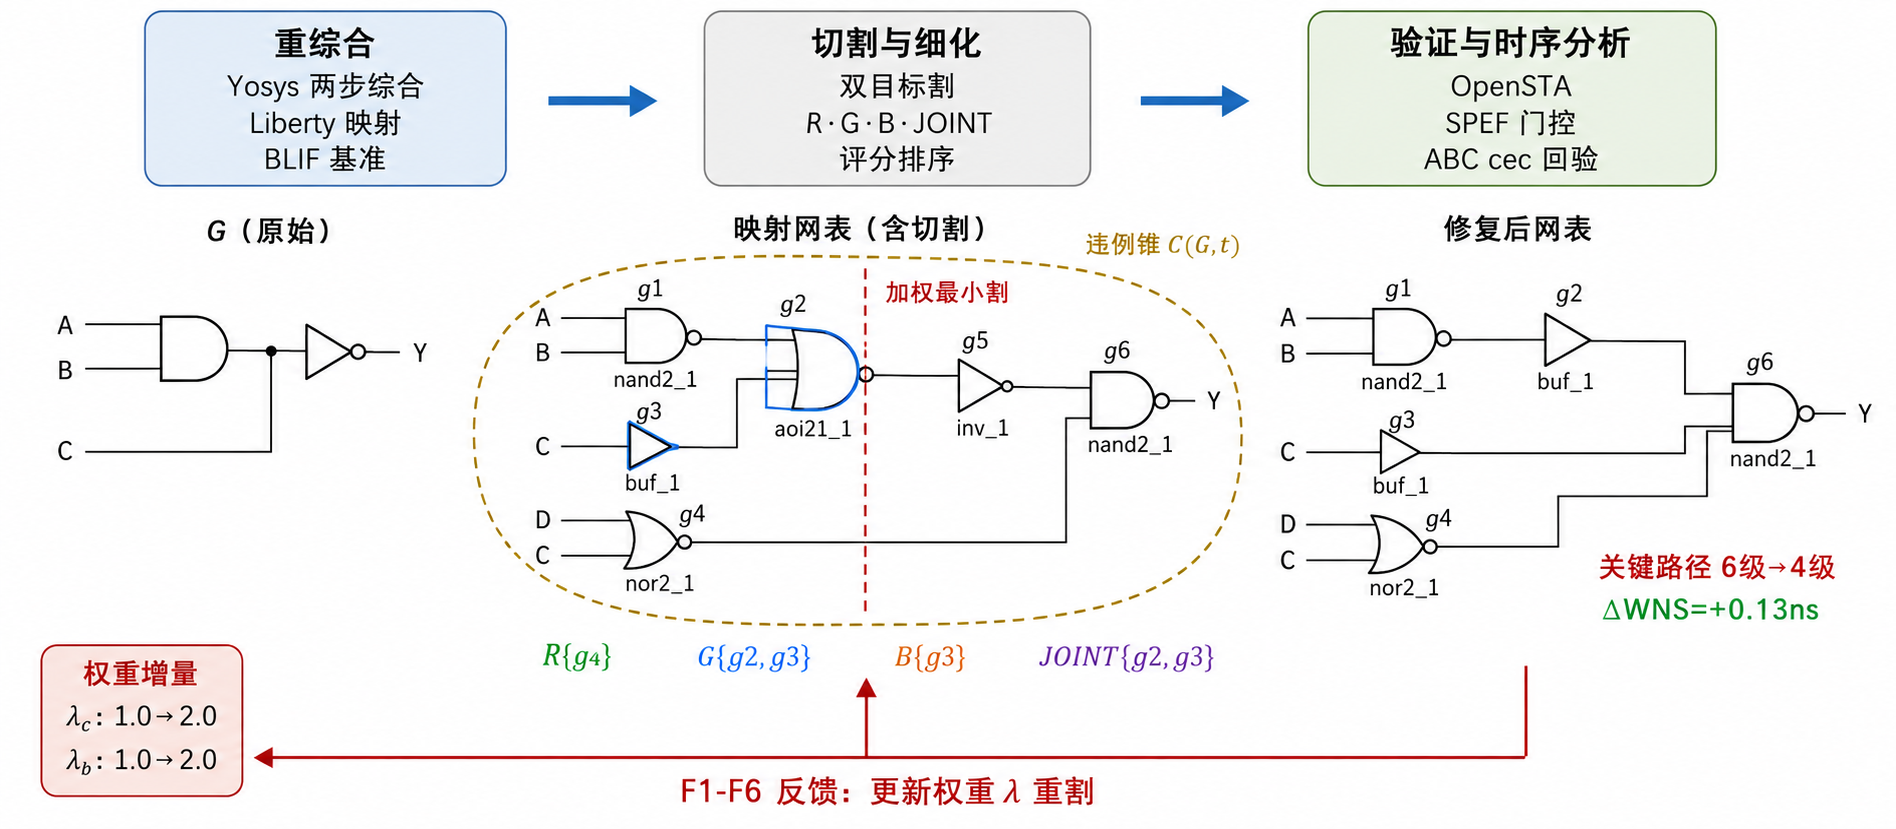
\includegraphics[width=0.92\textwidth]{fig3_method_flow_new.png}%
\caption{FAECO 三阶段流水线：映射网表准备 $\rightarrow$ 切割与候选细化 $\rightarrow$ 验证与时序分析。}
\label{fig:method_flow}
\end{figure*}

\begin{algorithm}[!t]
\footnotesize
\caption{FAECO 修复流程示意}\label{alg:main}
\begin{algorithmic}[1]
\Require 映射网表 $G'$、时序约束 $T$、工艺库 $\mathcal{L}$
\Ensure 修复后网表 $G^*$、接受候选集合 $\mathcal{A}$
\State 初始化 $G\gets G'$、$\mathcal{A}\gets\emptyset$ 和搜索权重 $\lambda$
\Repeat
  \State 从最差违例端点提取扇入锥，必要时按深度分治
  \State 构建加权割与关键路径覆盖割，生成并排序 R/G/B/JOINT 候选
  \State 对候选执行局部功能/结构检查和 OpenSTA 测量
  \State 对满足物理门控条件的候选进行简化 SPEF 复测
  \State 接受满足条件的候选并更新 $G,\mathcal{A}$；根据失败类型更新失败候选对应的 $\lambda$
\Until{无时序违例、候选耗尽或达到停止条件}
\State \Return $G,\ \mathcal{A}$
\end{algorithmic}
\end{algorithm}

算法~\ref{alg:main} 概括 FAECO 的主控制流：从最差违例端点提取并必要时分治扇入锥，生成和排序候选，依次完成局部功能/结构检查与时序测量；通过的候选更新网表，未通过的候选按失败类型反馈搜索权重。具体割图构建、策略实例化和失败类型定义见后文。

顺序实验的真实 STA 主流程采用局部功能/结构保持检查：R 的库函数匹配、G 的同功能尺寸替换、B 的恒等缓冲插入以及 JOINT 的组合均在候选构造时确定。当前主流程保留原始网表和重综合网表作为统一接口；候选级 ABC 的 \texttt{cec} 与顺序 SEC 作为独立验证接口，ABC 的 \texttt{cec} 用于组合网表回验。顺序主实验的 WNS 改善按构造级时序搜索结果报告。

本文将接受谓词明确写为 $A(p)=[\Delta_{\mathrm{WNS}}(p)>0]\lor[\mathrm{tns\_aware}\land\Delta_{\mathrm{WNS}}(p)=0\land\Delta_{\mathrm{TNS}}(p)>0]$；报告中逐项注明是否启用第二项。WNS 允许为正，实际终止条件是每轮候选耗尽后完成失败分类和权重更新，或达到 $r_{\max}$。实验中的 6 轮和 20 轮分别是运行配置，收敛行为由实测轨迹给出。

\FloatBarrier
\subsection{核心机制}\label{sec:mechanism}

\subsubsection{多特征加权割与候选优先级}
\begin{figure*}[t]
\centering
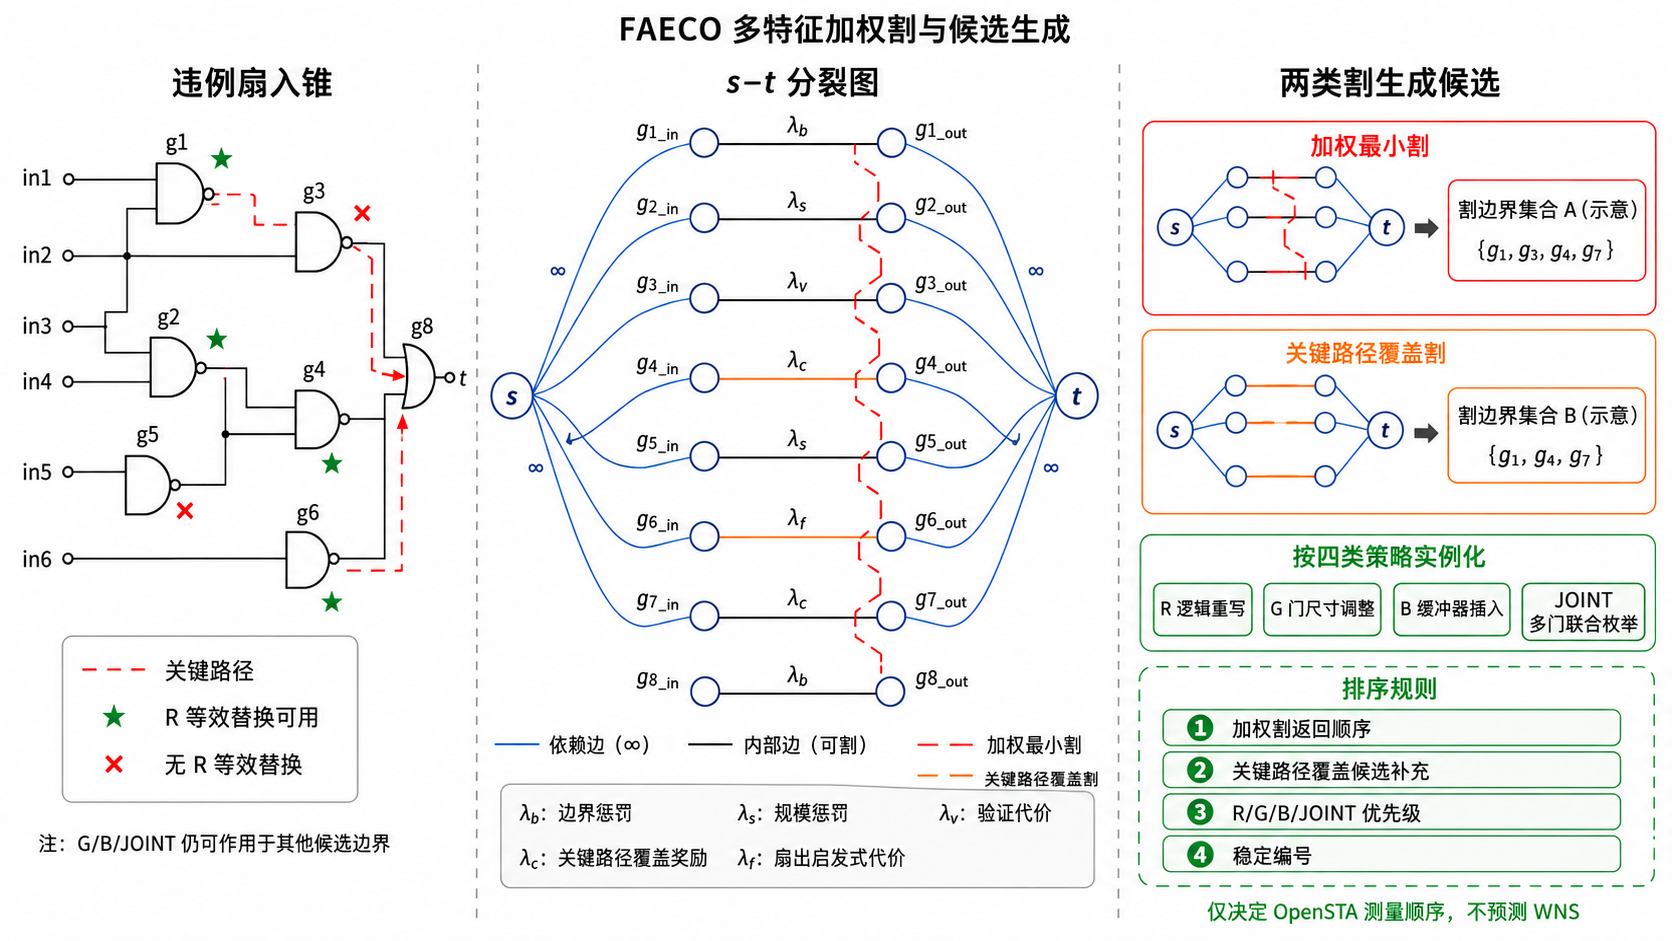
\includegraphics[width=0.68\textwidth]{fig_cut_generation_new.png}
\caption{多特征加权割与候选生成示意：扇入锥经 s-t 分裂后，加权最小割（红虚线）和关键路径覆盖割（橙虚线）形成两类割边界，再按四类策略实例化，并依据候选排序规则安排 OpenSTA 测量顺序；WNS 由 OpenSTA 实测得到}
\label{fig:cut_generation}
\end{figure*}

在扇入锥 $C(G, t)$ 上构建 s-t 分裂图 $K(G, t)$，定义见表~\ref{tab:symbols}、示意见图~\ref{fig:cut_generation}。每个门拆成输入/输出容量边，扇入依赖用无穷容量边，节点权重 $\mathrm{cost}(v)$ 与关键路径、层级、尺寸联动；全局最小割由 Edmonds-Karp 最大流算法\cite{edmondskarp} 求出，割边的源侧节点对应候选门。

分裂图复杂度为 $O(VE^2)$，其中顶点数 $V=2n+2$、$n$ 为锥内门数，边数 $E=O(n+f)$、$f$ 为扇入依赖边；数十万门级设计上单次割在数秒内完成。

候选构造和时序测量分别承担不同职责：局部功能保持规则约束可构造的替换类型，OpenSTA 再测量候选的真实时序收益。当前顺序主流程采用构造级筛选，全局 CEC/SEC 作为独立验证环节。

FAECO 将局部功能保持候选的可用性编码进割图：构建 $K(G, t)$ 时由 Liberty 文件中的布尔函数计算每个门的 R 候选集 $\mathcal{R}(v)$。对 $\mathcal{R}(v)=\emptyset$ 的不可替换门，其关键覆盖奖励置零并绑定 G/B 策略权重，使割集优先避开这类门。该机制约束候选构造空间，降低无效候选的预期比例；候选接受由 OpenSTA 实测决定，全局顺序 SEC 作为独立验证环节。

有 R 候选的门保留关键覆盖奖励，并按扇出数叠加扇出稳定性启发式代价；这里的扇出项不是已测得的等价验证概率。G/B 与 R 在同一割集方案中共同参与竞争，最终取舍由逐候选 OpenSTA 实测决定。

例如 b06 关键路径上的复合门均无 R 候选，关键覆盖奖励置零后割集方案只能生成 G/JOINT 候选，实验验证见 \S\ref{sec:itc99}。

候选接受阶段的实测 WNS 差定义为候选 $p$ 应用前后的 OpenSTA 差，在理想线网模式、同一时序约束文件（SDC）与时钟约束下计算：
\begin{equation}\label{eq:dtiming}
\Delta_{\mathrm{WNS}}(p) = \mathrm{WNS}_{\mathrm{after}}(p) - \mathrm{WNS}_{\mathrm{before}}.
\end{equation}
生成阶段使用已知图结构和启发式权重生成候选；OpenSTA 实测得到的 $\Delta_{\mathrm{WNS}}$ 用于接受和反馈。实际运行流程不计算独立的候选级 WNS 代理，而是先按加权割代价生成边界，再补充关键路径覆盖候选，并在边界内部按 R/G/B/JOINT 策略优先级排序。节点代价 $\mathrm{cost}(v)$ 是一组启发式代价：设 $\mathrm{depth}(v)$ 为 $v$ 在锥内的逻辑深度，则
{\small
\begin{equation}
\label{eq:cost}
\begin{aligned}
\mathrm{cost}(v) &= 1 + \frac{\lambda_b}{1+\mathrm{depth}(v)}
 + \lambda_s\,\frac{s(v)^2}{S} \\
&\quad + 0.01\lambda_v\,s(v)
 + 0.1\lambda_f\,\mathrm{fanout}(v),
\end{aligned}
\end{equation}
}
其中 $\lambda_b/\lambda_s/\lambda_v/\lambda_f$ 为边界、尺寸、验证和扇出启发式权重（默认均为 $1.0$），$\mathrm{fanout}(v)$ 为门 $v$ 的扇出数（仅对有 R 候选的门计入），$s(v)$ 为门 $v$ 的扇入锥规模，$S=\sum_u s(u)^2$ 为平方和。关键路径覆盖不是式~\eqref{eq:cost} 中的连续预测项，而是由独立的关键路径覆盖候选和 $\lambda_c$ 反馈控制。

归一化项引导割集避开锥规模过大的门，验证代价项由 F5 反馈上调，扇出项由稳定性启发式控制，关键路径覆盖候选由 $\lambda_c$ 反馈调节；式~\eqref{eq:cost} 用于候选边界生成，WNS 由 OpenSTA 实测。

候选优先级由三层确定：加权割返回顺序、关键路径覆盖候选的补充顺序，以及 R/G/B/JOINT 策略优先级和稳定编号，作用是安排 OpenSTA 的测量顺序。27 次与 110 次的差异反映候选排序与提前停止带来的测量次数变化。

\subsubsection{失效驱动细化}
\begin{figure*}[t]
\centering
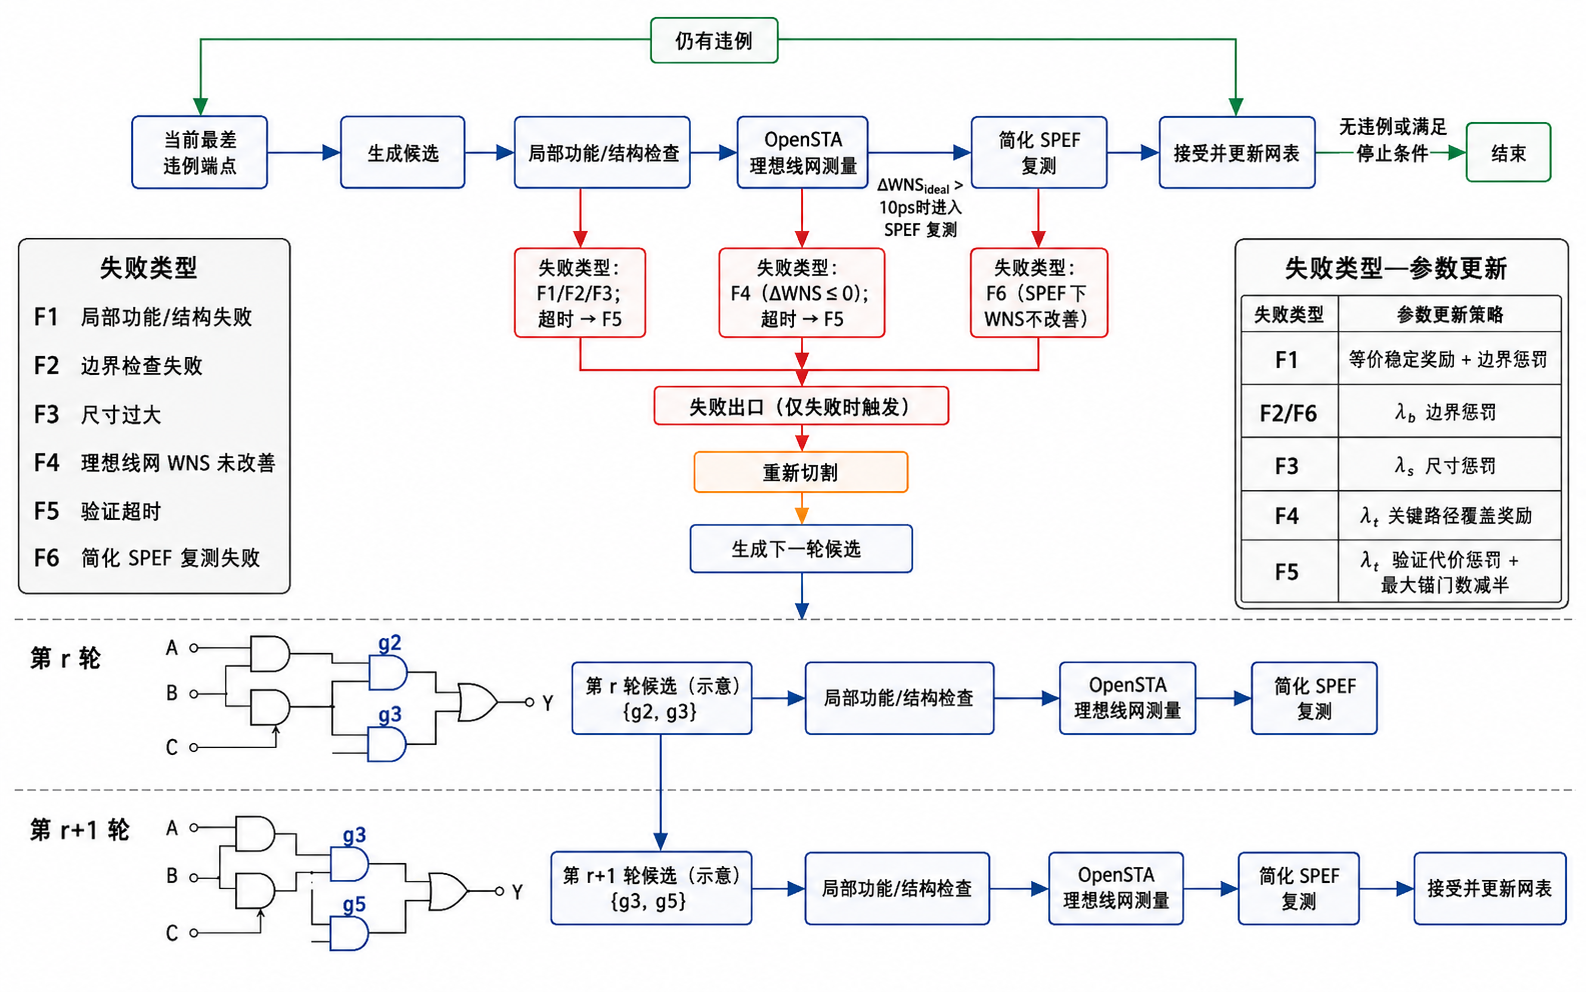
\includegraphics[width=0.82\textwidth]{fig_feedback_loop_new.png}
\caption{F1--F6 失效驱动反馈闭环：候选实测失败后按类型更新割权重并重割，直至接受或达到轮数上限}
\label{fig:feedback_loop}
\end{figure*}

F1--F6 失败分类驱动细化（表~\ref{tab:failures}，流程见图~\ref{fig:feedback_loop}）。多轮细化按“割图、失败分类、权重更新、重割”循环，直至成功或达到最大迭代数；关闭反馈（固定权重）作为消融对照。对于顺序实验的真实 STA 主流程，设计上 F1 对应候选构造阶段的局部功能/结构筛选，F4 对应理想线网 WNS 未改善，F6 对应 SPEF 复测未改善；三者的检测路径与组合网表的全局 CEC 不同。现有外层循环的 JSON 记录中可直接追溯的失败类型包括 F3、F4 和 F6；F1/F2/F5 的接口和阈值已实现，发生率统计作为后续审计项。

权重更新不是简单重试，而是每次失败将对应权重增加 $1.0$，默认初值均为 $1.0$：F1 提高等价稳定奖励并增加边界惩罚 $\lambda_b$，F2/F6 增加边界惩罚 $\lambda_b$，F3 增加尺寸惩罚 $\lambda_s$，F4 增加关键覆盖奖励 $\lambda_c$，F5 增加验证代价惩罚 $\lambda_v$ 并将最大锥门数减半，下限为 1；例如 F4 连续两次触发后 $\lambda_c$ 由 $1.0$ 增至 $3.0$，关键路径门的割代价随之降低。效果示例见 \S\ref{sec:ablation}。

\begin{table}[ht]
\centering
\caption{F1--F6 失败类型与反馈动作}
\label{tab:failures}
\scriptsize
\setlength{\tabcolsep}{2pt}
\begin{tabular}{p{2.0cm}p{2.6cm}p{2.9cm}}
\toprule
\textbf{失败类型} & \textbf{检测条件} & \textbf{反馈动作} \\
\midrule
F1 局部功能/结构失败 & Liberty 文件中的函数匹配或结构检查未通过 & 提高等价稳定奖励并增加边界惩罚，使此类候选在下一轮割代价中贬值 \\
F2 边界失败 & 锥边界未闭合 & 增加边界惩罚 $\lambda_b$，收紧锥边界，保留已映射门 \\
F3 尺寸过大 & 候选尺寸超过阈值 & 增加尺寸惩罚，强制更小割 \\
F4 时序收益不足 & $\Delta_{\mathrm{WNS}} \leq 0$（建立时间模式） & 上调关键覆盖奖励，使下一轮割集方案集中于真实关键路径门 \\
F5 验证超时 & 局部检查或 STA 运行时间 $>60\,$s & 增加验证代价惩罚 $\lambda_v$ 并将最大锥门数减半 \\
F6 SPEF 复测失败 & 理想线网增益 $>10\,$ps 但 SPEF 下 WNS 不改善 & 标记高线载路径，增加边界惩罚以规避高扇出路径 \\
\bottomrule
\end{tabular}
\end{table}

\subsubsection{形式等价与门控验证}
候选级功能保持在生成期由 Liberty 文件中的函数匹配和结构规则保证，时序指标由 OpenSTA 3.1.0 在理想线网模式下实测得到。

代码保留独立组合网表的 ABC \texttt{cec} 回验接口（Yosys 归一化后调用 ABC）；当前顺序实验的真实 STA 主循环由 OpenSTA 实测主导，单次约为 $0.3$--$4\,$s。本实验报告构造级时序搜索结果，顺序 SEC 作为独立验证接口。

\begin{figure}[!t]
\centering
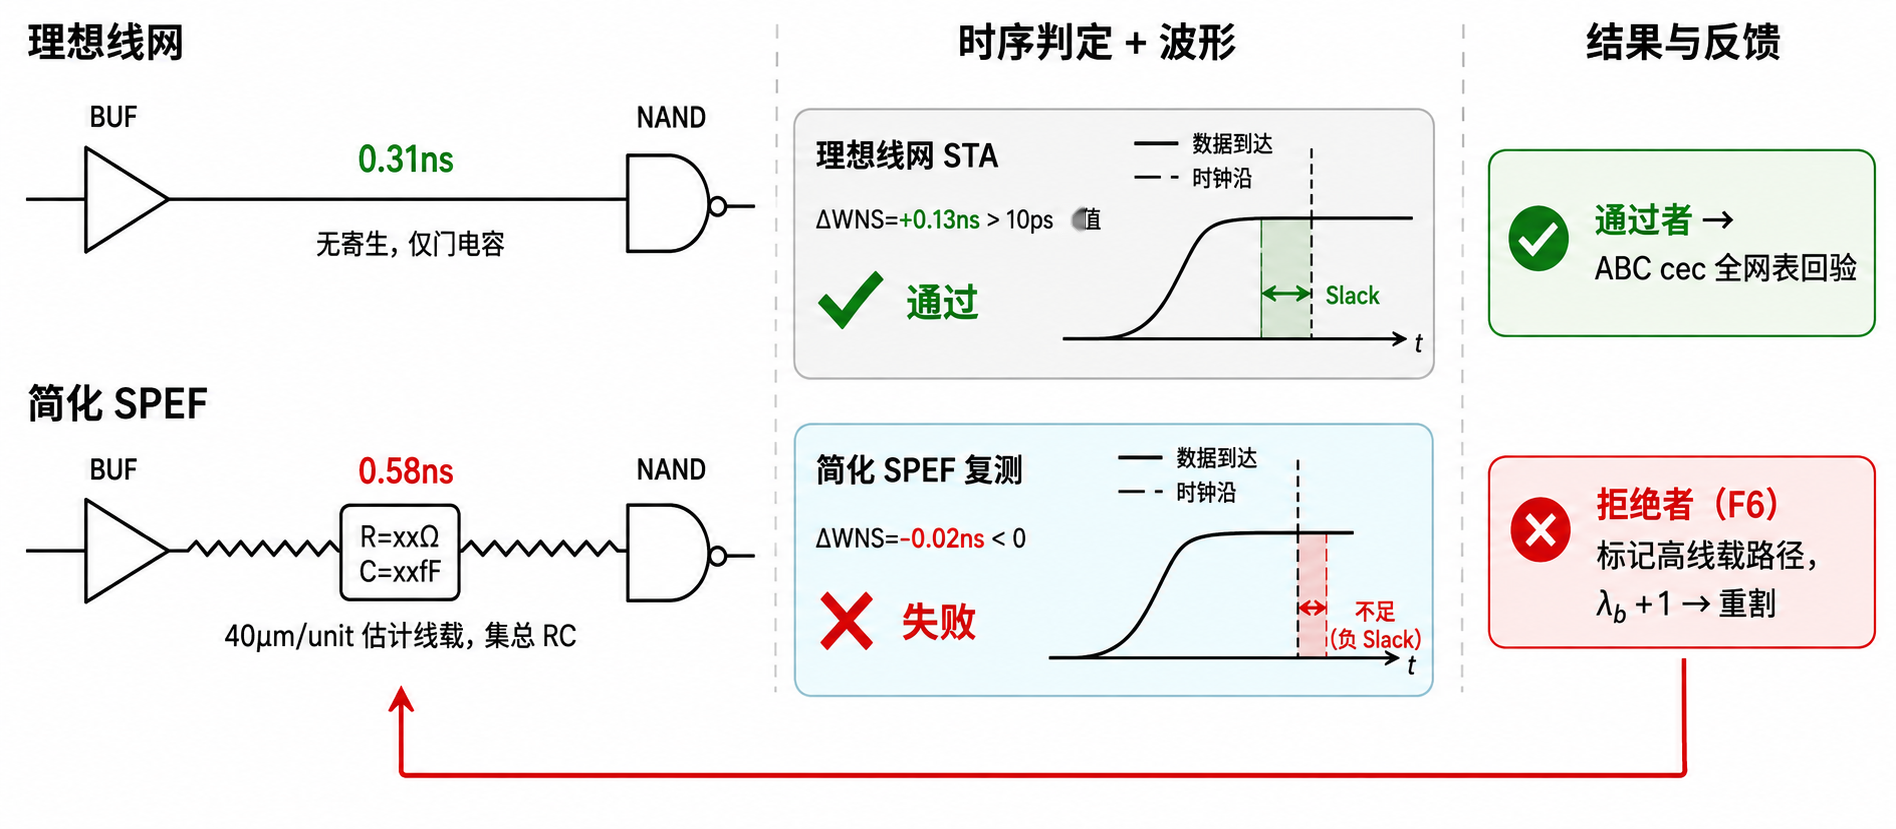
\includegraphics[width=1.0\columnwidth]{fig_spef_gate_new.png}
\caption{简化 SPEF 门控的两层验证流程：候选先由 OpenSTA 在理想线网模式下实测，改善超过阈值才进入简化 SPEF 复测，复测仍严格改善才接受；未通过者归类为 F6 反馈，并上调边界惩罚后重新分割}
\label{fig:spef_gate}
\end{figure}

该门控将一次线载复测纳入内层循环；相关参数尚未完成工艺校准，实验中的门控候选均未通过。当前门控用于筛除物理无效候选，物理保持性由真实布局布线结果核验，召回率需在参数校准后评估。

\FloatBarrier
\subsection{工程实现要点}\label{sec:impl}

为生成映射网表，实验采用 Yosys 的 \texttt{synth -noabc} 与 \texttt{abc -liberty} 两步流程；FAECO 本身在已映射的 SKY130 HD 网表上执行 R/G/B/JOINT 局部候选搜索。工艺库、输入 Verilog 文件和脚本版本均固定，实验适用范围为该工具链、工艺角和顺序约束；多工艺、多角及顺序 SEC 属于扩展验证场景。

扇入锥 $C(G, t) = (V_C, E_C)$ 由反向广度优先搜索（BFS）抽取。对数十万门设计，按逻辑深度将违例锥切分为受门数上限限制的子锥，独立抽取候选并沿关键路径顺序生成，使候选集中于关键路径并控制内存与求解规模。上述设计在第~\ref{sec:exp} 节依次验证：主结果检验修复质量与效率，跨测试集检验可迁移表现，消融与基线对比检验联合系统行为，真实版图验证检验版图后保持性与 SPEF 门控边界。

% =============================================================================
% IV. 实验
% =============================================================================
\FloatBarrier
\section{实验}\label{sec:exp}

\subsection{实验设置}\label{sec:setup}

\textbf{环境与数据集}：实验使用 OSS-CAD Suite（Yosys 0.67+146）、OpenSTA 3.1.0\cite{opensta}、Z3 5.0.0\cite{z3}、NetworkX 3.6.1\cite{networkx} 与 Python 3.11.9，运行于 WSL2 Ubuntu（8 核 16 线程、32 GB RAM）；固定工具链版本和随机种子以保证流程确定性。主实验采用 8 个 ISCAS89 顺序电路，经 Yosys 映射至 SKY130 HD 标准单元库，并由 OpenSTA 在 0.5 ns 时钟周期下构造时序违例；ITC-99 与 PicoRV32 用于跨测试集评估，见 \S\ref{sec:itc99}、\S\ref{sec:ood}。质量指标为理想线网 WNS/TNS 与布线后 WNS，效率指标为候选级 STA 测量次数；“严格改善”表示建立时间 WNS 增大（包括由负转正），SPEF 复测和实际运行时间不计入上述 STA 测量次数。

\textbf{配置与参数}：所有电路使用统一流程，分别运行效率优先与收敛两种配置：前者搜索宽度为 $w=1$、最多 10 轮，并在首个严格改善后停止；后者最多 20 轮，直至没有满足接受条件的候选。真实顺序 STA 主流程每轮默认评估 8 个候选、最多作用于 8 个关键实例，反馈最多触发 6 轮；收敛实验采用 20 轮外层配置。JOINT 沿关键路径深度至多 3 的滑动窗口枚举（上限 50 个组合，不含 B），扇入锥分治阈值为 1000 门。F3、F5 的默认阈值分别为 15\% 和 60 s，物理门控阈值为 10 ps 理想线网增益，估计线长单位为 40\,$\mu$m/unit；这些参数分别对应结构筛选、运行时反馈和物理筛选，接受条件由 OpenSTA 实测定义。27/110 为历史批次的候选级 STA 调用数。

\subsection{主结果：ISCAS89 修复质量与效率}\label{sec:iscas}

图~\ref{fig:iscas_main} 与表~\ref{tab:pr8} 所示的 8 个 ISCAS89 基线--修复网表配对结果，在预布局理想线网模式下经 OpenSTA 测量均实现严格改善；修复候选由 \texttt{manifest.json} 指定，来自不改写 D 触发器、时钟和复位的 R/G/B/JOINT 构造级保持变换。当前顺序主实验采用构造级保持检查，本节报告时序搜索结果，独立形式验证属于后续验证环节。策略分布方面：JOINT 候选对应 s27/s382/s420/s953，G 对应 s641/s713/s832，R 对应 s820；B 的建立时间收益见附录，不纳入本组建立时间配对结果。该配对结果与后文 20 轮收敛实验及效率优先历史批次分开统计。

从机制上看，JOINT 沿关键路径压缩多级逻辑深度，单门 G 只调整驱动强度而不改变逻辑级数；R 依赖工艺库中的等价布尔候选，在 ISCAS89 中的覆盖有限，这与 \S\ref{sec:itc99} 中 b06 未达到严格改善的情况具有相同原因。

\begin{figure}[!t]
\centering
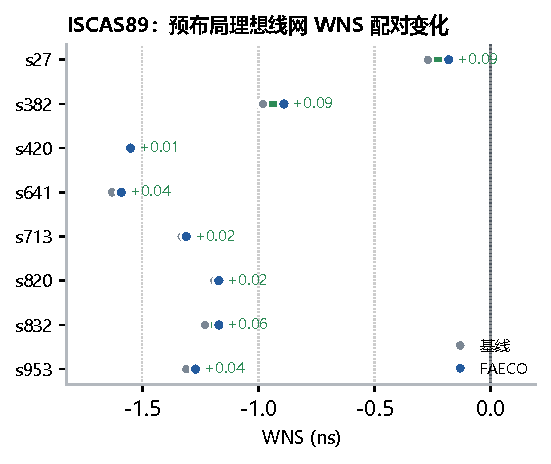
\includegraphics[width=1.0\columnwidth]{fig_iscas89.pdf}
\caption{ISCAS89 顺序电路混合修复的基线--FAECO 配对结果（周期 0.5 ns；标注为 FAECO 相对基线的 WNS 变化）}
\label{fig:iscas_main}
\end{figure}

\subsection{跨测试集评估}\label{sec:ood}

\subsubsection{ITC-99 基准族}\label{sec:itc99}

在 19 个可映射到 SKY130 HD 的 ITC-99 电路中，18 个电路的 WNS 严格改善（94.7\%），剩余的 b06 与基线持平。因此，19 个电路均未出现 WNS 回退，其中六个大规模电路 b14/b15/b17/b20/b21/b22 均成功（图~\ref{fig:itc99}）。该结果刻画了同一工艺库和时序约束下的跨测试集表现；跨工艺泛化需在其他工艺库上单独评估。b06 是唯一未达到严格改善的电路：其关键路径由缺少等价 R 候选的复合门链构成，G 放大与 JOINT 枚举均因输入电容增大而拖累前级，纯 G 与混合策略的候选全部被拒（分别为 148 次和 156 次）。

策略分布以 JOINT 为主（12 个，b20/b21 的收益最大，分别为 $+1.98$ 和 $+2.16\,$ns）；19 个电路共进行 1693 次候选级 STA 测量，实际运行时间约 12.5 分钟。

独立大电路补充实验单独统计 b18 与 b19：两者分别含 37.6 万和 75.5 万个门，在同一 Yosys 0.67 工具链下分别经过 93 次和 58 次候选级 STA 测量完成修复；门数相对 ISCAS89 增大数千倍，单个电路的 STA 测量次数仍为数十次量级，与 ISCAS89 效率优先配置（8 个电路合计 27 次）同量级，当前样本中的测量次数未随门数呈指数增长。

\begin{figure*}[t]
\centering
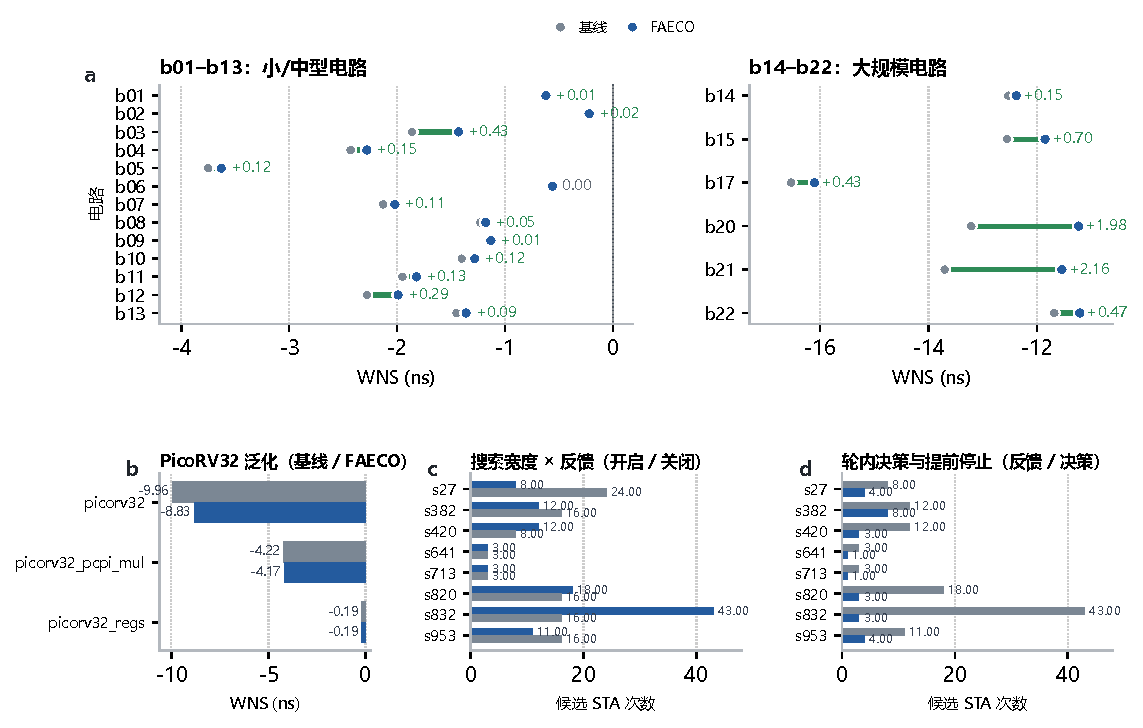
\includegraphics[width=0.96\textwidth]{fig_cross_eval.pdf}
\caption{跨测试集评估与消融效率。a，ITC-99 电路按规模分面的基线--FAECO 配对 WNS；b，PicoRV32 三个子模块的 WNS；c，反馈开关对候选级 STA 次数的影响；d，轮内决策与提前停止对候选级 STA 次数的影响。}
\label{fig:itc99}
\end{figure*}

\subsubsection{PicoRV32 异构族}

基于同一寄存器传输级（RTL）源的三个结构差异明显子模块直接复用 ISCAS89 流程（图~\ref{fig:itc99}b）：PicoRV32 与 pcpi\_mul 分别经 R、G 获得 $+1.13$ 和 $+0.05\,$ns 的改善，存储密集子模块未改善，构成与 b06 类似的结果边界。

\subsection{消融与基线对比}\label{sec:ablation}

本小节分别去除反馈、决策层和候选空间，检验各机制对质量与效率的贡献。

\textbf{质量}：收敛配置下，混合策略在 8 个电路中均优于纯 G 和随机基线，并在 7 个电路中严格优于纯 B（图~\ref{fig:baseline}、表~\ref{tab:min_trials}；表中 STA 列为达到各自最终 WNS 的累计候选级 STA 测量次数）。混合策略的平均改善为 1.07 ns，纯 G 为 0.16 ns；中位数分别为 1.13 ns 和 0.09 ns。随机基线与混合策略共享 R/G 子空间，未启用 B/JOINT。

\begin{figure}[!t]
\centering
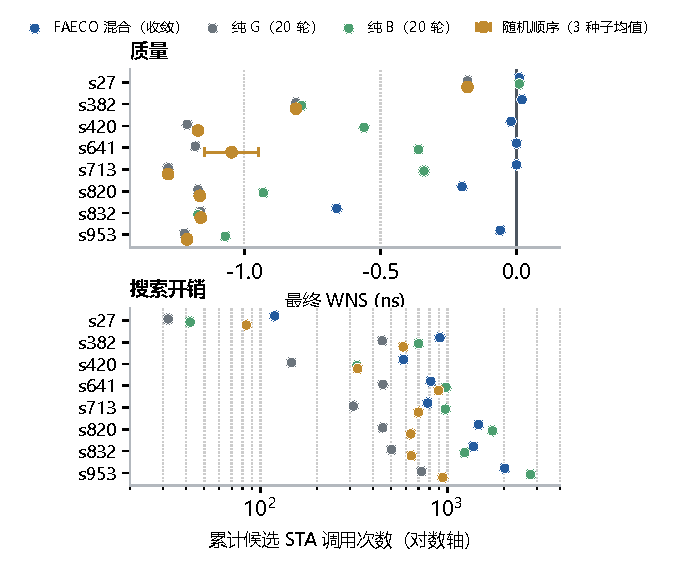
\includegraphics[width=1.0\columnwidth]{fig_baseline.pdf}
\caption{收敛配置竞争基线对比：左为最终 WNS 点图（随机基线带 3 个随机种子的标准差），右为累计候选级 STA 测量次数点图；右图横轴为对数轴}
\label{fig:baseline}
\end{figure}

\textbf{效率}：反馈开启将所需搜索宽度从 $\geq 4$--$8$ 降至 $\leq 2$，STA 开销节省 $44\%$--$89\%$（图~\ref{fig:itc99}b）；一批效率优先的历史实验在 8 个电路上记录了合计 27 次候选级 STA 测量，另一独立的全候选批次记录 110 次，测量次数差异为 75.5\%。留一法评估在 8 个电路上全部成功；两批次的候选全集、排序版本和完整命令行未统一保存，27/110 作为描述性测量开销报告。

收敛配置的累计 STA 开销见表~\ref{tab:min_trials}（混合 8069 次、纯 G 约 3066 次、随机约 4800 次）；该组数据用于质量收敛曲线，效率优先模式单独报告调用次数。27 次与 110 次均统计理想线网 STA 测量，不含局部检查、SPEF 复测和实际运行时间。同预算对照（s382/s820，60/500 次 STA）中，固定与随机两种非自适应顺序最终 WNS 一致；结果显示候选排序与提前停止能够减少测量次数。

\textbf{策略与鲁棒性}：纯策略消融（图~\ref{fig:ablation}）表明，B 单独使用的收益不超过 0.06 ns（ISCAS89 无净改善，ITC-99 中 11/19 个电路小幅提升），混合收益由 R/G/JOINT 承担；不同电路的单一策略表现存在差异，例如 s382 的纯 R 失败，而 b15 和 PicoRV32 的单一策略已达到混合策略水平。

参数敏感性方面，SPEF 复测阈值（5/10/20 ps）与 s382 权重扰动（$\pm 100\%$）均不改变结论；热启动相较冷启动减少近一半的 STA 开销，代表性收敛轨迹见图~\ref{fig:convergence}。

\begin{figure}[!t]
\centering
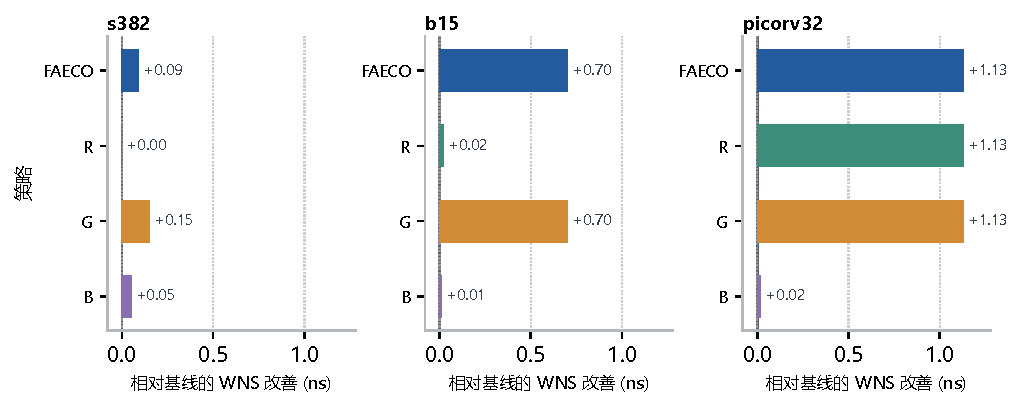
\includegraphics[width=1.0\columnwidth]{fig_ablation.pdf}
\caption{纯策略消融：三类电路上各策略相对基线的 WNS 改善（混合含 R/G/B/JOINT，窗口深度 3）}
\label{fig:ablation}
\end{figure}

\begin{figure}[!t]
\centering
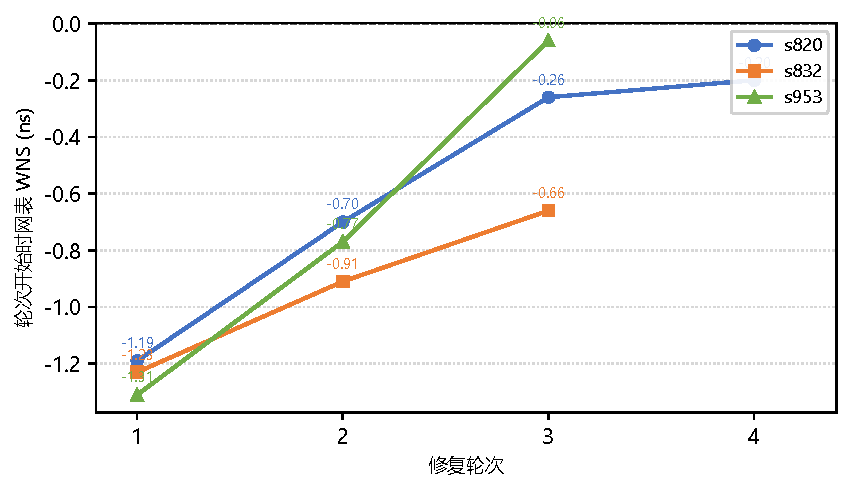
\includegraphics[width=1.0\columnwidth]{fig_convergence.pdf}
\caption{收敛配置下 WNS 随外层循环轮次变化（每轮至多接受一个候选，数据点为轮开始时的网表 WNS）}
\label{fig:convergence}
\end{figure}

\begin{table}[ht]
\centering
\caption{不同策略在收敛配置（20 轮）下的最终 WNS 与 STA 开销，WNS 单位 ns}
\label{tab:min_trials}
\setlength{\tabcolsep}{2pt}
\footnotesize
\begin{tabular}{lrrrrrrrr}
\toprule
\textbf{电路} & \textbf{混合} & \textbf{混合} & \textbf{纯 G} & \textbf{纯 G} & \textbf{纯 B} & \textbf{纯 B} & \textbf{随机} & \textbf{随机} \\
 & \textbf{WNS} & \textbf{STA} & \textbf{WNS} & \textbf{STA} & \textbf{WNS} & \textbf{STA} & \textbf{WNS} & \textbf{STA} \\
\midrule
s27  & $+0.01$ & 119  & $-0.18$ & 32  & $+0.01$ & 42  & $-0.18$ & 84 \\
s382 & $+0.02$ & 910  & $-0.81$ & 447 & $-0.79$ & 700 & $-0.81$ & 578 \\
s420 & $-0.02$ & 580  & $-1.21$ & 146 & $-0.56$ & 328 & $-1.17$ & 330 \\
s641 & $0.00$  & 814  & $-1.18$ & 451 & $-0.36$ & 980 & $-1.05$ & 894 \\
s713 & $0.00$  & 784  & $-1.28$ & 313 & $-0.34$ & 974 & $-1.28$ & 699 \\
s820 & $-0.20$ & 1464 & $-1.17$ & 450 & $-0.93$ & 1740 & $-1.16$ & 635 \\
s832 & $-0.66$ & 1375 & $-1.16$ & 501 & $-1.17$ & 1236 & $-1.16$ & 640 \\
s953 & $-0.06$ & 2023 & $-1.22$ & 726 & $-1.07$ & 2782 & $-1.21$ & 944 \\
\bottomrule
\multicolumn{9}{p{0.95\columnwidth}}{\footnotesize STA 为达到各自最终 WNS 的累计候选级 STA 测量次数；随机基线在 R/G 子空间内随机排序，未启用 B/JOINT，其 WNS 与 STA 为 3 个随机种子的均值。}\\
\end{tabular}
\end{table}

\subsection{物理验证：版图保持性与 SPEF 门控}\label{sec:phys_closure}

在真实布局布线（placement and routing，P\&R）后，8 个 ISCAS89 电路中有 5 个电路仍保持时序改善，1 个持平，2 个轻微恶化但不超过 0.02 ns（图~\ref{fig:pr_delta}、表~\ref{tab:pr8}）。该批次的 16 份预布局 STA 日志、16 份布线运行日志和 16 份最终数据库文件 \texttt{final.odb} 已归档，预布局汇总见 \texttt{pre\_layout\_audit\_summary.json}；流程使用 OpenROAD 2.0、SKY130 HD 和 0.5 ns 时钟约束，并在全局布线估计寄生后进行时序对比。本节给出布线后时序核验，DRC 报告未生成。另设两组独立实验，均使用同一电路的配对基线/修复网表：（A）SPEF 负载扫描，量化候选的物理保持边界；（B）迭代式 SPEF 门控，将 F6 复测失败接入权重更新。

\begin{table}[ht]
\centering
\caption{真实布局布线后的版图验证：8 个 ISCAS89 电路布线后 WNS 对比（OpenROAD 2.0 + SKY130 HD）}
\label{tab:pr8}
\footnotesize
\setlength{\tabcolsep}{2pt}
\begin{tabular}{lrrrrr}
\toprule
\textbf{电路} & \textbf{预布局基线} & \textbf{预布局修复} & \textbf{布线后基线} & \textbf{布线后修复} & $\Delta$ \\
\midrule
s27  & $-0.27$ & $-0.18$ & $-0.36$ & $-0.22$ & $+0.14$ \\
s382 & $-0.98$ & $-0.89$ & $-1.16$ & $-1.02$ & $+0.14$ \\
s420 & $-1.56$ & $-1.55$ & $-1.80$ & $-1.82$ & $-0.02$ \\
s641 & $-1.63$ & $-1.59$ & $-2.10$ & $-2.02$ & $+0.08$ \\
s713 & $-1.33$ & $-1.31$ & $-1.59$ & $-1.58$ & $+0.01$ \\
s820 & $-1.19$ & $-1.17$ & $-1.52$ & $-1.49$ & $+0.03$ \\
s832 & $-1.23$ & $-1.17$ & $-1.51$ & $-1.51$ & $0.00$ \\
s953 & $-1.31$ & $-1.27$ & $-1.60$ & $-1.61$ & $-0.01$ \\
\bottomrule
\multicolumn{6}{p{0.92\columnwidth}}{\footnotesize 统一映射网表与同一接受候选；s27 因面积过小采用 10\% 利用率布局规划；布线后 $\Delta$ 为修复网表相对基线网表的 WNS 变化；DRC 签核需另行统计。}\\
\end{tabular}
\end{table}

\begin{figure}[!t]
\centering
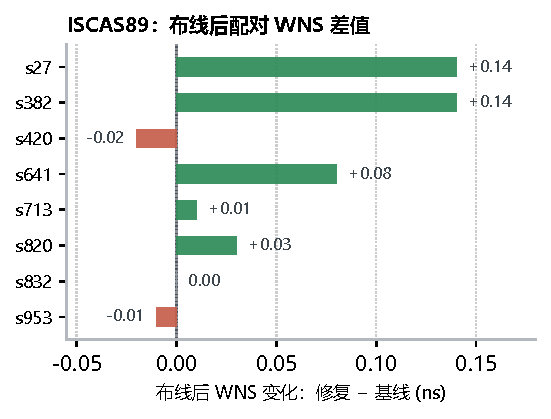
\includegraphics[width=1.0\columnwidth]{fig_pr_delta.pdf}
\caption{8 个 ISCAS89 电路布线后 WNS 的配对差值；正值表示修复网表相对基线网表改善，负值表示轻微回退}
\label{fig:pr_delta}
\end{figure}

（A）\textbf{独立 SPEF 负载扫描}：s382 的 R 候选与 b18 的 JOINT 候选的 WNS 改善随估计线长增大而归零（图~\ref{fig:spef}），说明理想线网候选存在物理保持边界。

\begin{figure}[!t]
\centering
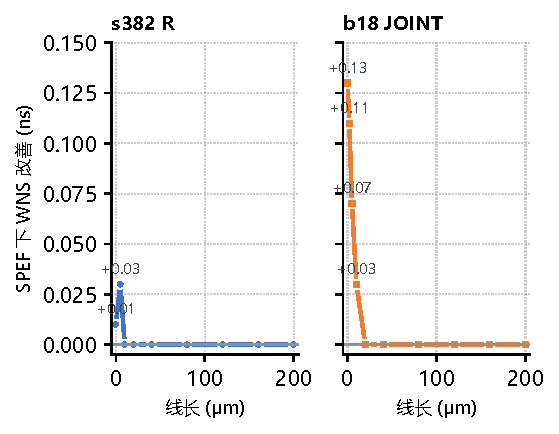
\includegraphics[width=1.0\columnwidth]{fig_spef.pdf}
\caption{SPEF 负载扫描下 WNS 随线长的变化（s382-R 与 b18-JOINT；两面板同轴范围）}
\label{fig:spef}
\end{figure}

（B）\textbf{迭代式门控}：对主实验收集的理想线网改善候选执行两层门控复测，s382 的 50 个与 b18 的 6 个候选在 40\,$\mu$m/unit 估计线载下全部未通过，未通过的候选按 F6 反馈更新权重；当前线长估计采用保守设置，物理候选召回率需通过真实布局布线结果评估。门控参数（复测阈值 10 ps、线长 40\,$\mu$m/unit）仍待工艺校准，当前门控用于筛除物理无效候选，参数校准列为后续工作，见 \S\ref{sec:conclusion}。

B 策略在受控保持时间场景下的补充验证见\mbox{附录~\ref{app:hold}}。
\FloatBarrier
\newpage
\section{结论}\label{sec:conclusion}

本文以失效驱动的多特征加权割与反馈重切为设计核心，通过将局部功能保持可用性、关键路径覆盖和候选规模编码进割权重，并依据实测失败类型更新权重，解决了预布局门级时序 ECO 中深层逻辑候选难生成、功能约束与时序收益难协调的问题。在公开 SKY130 HD 工具链上，FAECO 在 ISCAS89、ITC-99 和 PicoRV32 上分别实现 8/8、18/19 和 2/3 个电路的严格 WNS 改善；收敛配置下混合策略平均改善 1.07\,ns（纯 G 为 0.16\,ns），反馈开启后 STA 开销节省 44\%--89\%，布局布线后 8 个 ISCAS89 电路中 5 个保持改善、1 个持平，验证了机制的有效性。该方法适用于固定工艺库和时序约束下的预布局已映射门级 ECO，效果依赖库内等价候选、理想线网 STA 以及 SPEF 线长估计；对缺少 R 等价候选且 G/JOINT 会拖累前级的电路，修复能力受限。未来工作将校准物理门控模型并扩展至多工艺和全局顺序等价验证。




\clearpage
\onecolumn
\appendix
\section{保持时间补充数据}\label{app:hold}

作为补充场景，在 \texttt{set\_clock\_uncertainty -hold 0.8\,ns} 约束下测试 B 策略对最差保持松弛路径的修复：7/8 个电路获得可由真实 STA 测得的收益，s820/s832 修至满足时序，其余电路改善 $0.01$--$0.05\,$ns，且均未劣化建立时间 WNS。其机理在于 D 端轻负载的缓冲器链直接增加数据路径延迟；s27 因 D 端负载已较轻而未获得净收益。B 在建立时间场景下收益可忽略（ISCAS89 上无净改善），二者共同说明了 B 的适用场景边界。

\begin{table}[H]
\centering
\caption{保持时间场景扩展：B 策略迭代修复的真实 OpenSTA 实测（\texttt{set\_clock\_uncertainty -hold 0.8\,ns}）}
\label{tab:hold}
\small
\setlength{\tabcolsep}{2pt}
\begin{tabular}{lrrrp{9.2cm}}
\toprule
\textbf{电路} & \textbf{保持基线} & \textbf{修复后} & \textbf{建立 WNS} & \textbf{修复动作} \\
\midrule
s382 & $-0.38$ & $-0.33$ & $-0.98$ & 2 轮：DFF\_2 / DFF\_13 各 1$\times$buf\_1 \\
s420 & $-0.36$ & $-0.33$ & $-1.56$ & 1 轮：DFF\_12 1$\times$buf\_1 \\
s641 & $-0.36$ & $-0.35$ & $-1.63$ & 1 轮：DFF\_4 1$\times$buf\_1 \\
s713 & $-0.36$ & $-0.35$ & $-1.33$ & 1 轮：DFF\_15 1$\times$buf\_1 \\
s820 & $-0.16$ & $+0.01$（满足时序） & $-1.19\rightarrow -1.12$ & 4 轮：DFF\_0/1/3/2 各 1$\times$buf\_1 \\
s832 & $-0.08$ & $+0.01$（满足时序） & $-1.23\rightarrow -1.16$ & 4 轮：DFF\_3/0/2/1 各 1$\times$buf\_1 \\
s953 & $-0.22$ & $-0.20$ & $-1.31$ & 2 轮：DFF\_1 / DFF\_19 各 1$\times$buf\_1 \\
s27 & $-0.36$ & $-0.36$（无改善） & $-0.27$ & ---（4 候选全被拒绝） \\
\bottomrule
\end{tabular}
\end{table}


\clearpage
\twocolumn
\renewcommand{\refname}{参考文献}
\ctexset{section = {format=\heiti\fontsize{10.5}{14}\selectfont}}
\footnotesize
\begin{thebibliography}{99}
\bibitem{ho2010eco} Ho K H, Chen Y P, Fang J W, et al. ECO timing optimization using spare cells and technology remapping[J]. IEEE Transactions on Computer-Aided Design of Integrated Circuits and Systems, 2010, 29(5): 697-710.
\bibitem{ho2012treco} Ho K H, Jiang J H R, Chang Y W. TRECO: Dynamic technology remapping for timing engineering change orders[J]. IEEE Transactions on Computer-Aided Design of Integrated Circuits and Systems, 2012, 31(11): 1723-1733.
\bibitem{kravets2019symbolic} Kravets V N, Lee N Z, Jiang J H R. Comprehensive search for ECO rectification using symbolic sampling[C]//Proceedings of the 56th Annual Design Automation Conference. New York: ACM, 2019: 1-6.
\bibitem{chen2012fixability} Chang H Y, Jiang I H R, Chang Y W. Timing ECO optimization via Bezier curve smoothing and fixability identification[J]. IEEE Transactions on Computer-Aided Design of Integrated Circuits and Systems, 2012, 31(12): 1857-1866.
\bibitem{chen2012metal} Chang H Y, Jiang I H R, Chang Y W. Timing ECO optimization using metal-configurable gate-array spare cells[C]//Proceedings of the 49th Annual Design Automation Conference. New York: ACM, 2012: 802-807.
\bibitem{jiang2010fraig} Wu B H, Yang C J, Huang C Y, et al. A robust functional ECO engine by SAT proof minimization and interpolation techniques[C]//Proceedings of IEEE/ACM International Conference on Computer-Aided Design. Piscataway: IEEE, 2010: 729-734.
\bibitem{lin2011simult} Chang H Y, Jiang I H R, Chang Y W. Simultaneous functional and timing ECO[C]//Proceedings of the 48th Annual Design Automation Conference. New York: ACM, 2011: 140-145.
\bibitem{jiang2016resource} Cheng A C, Jiang I H R, Jou J Y. Resource-aware functional ECO patch generation[C]//Proceedings of the Design, Automation \& Test in Europe Conference. Piscataway: IEEE, 2016: 1036-1041.
\bibitem{luo2016unified} Hung J H, Lin Y C, Cheng W K, et al. Unified approach for simultaneous functional and timing ECO[J]. IET Circuits, Devices \& Systems, 2016, 10(6): 514-521.
\bibitem{zhuo2018patch} Dao A Q, Lee N Z, Chen L C, et al. Efficient computation of ECO patch functions[C]//Proceedings of the 55th Annual Design Automation Conference. New York: ACM, 2018: 1-6.
\bibitem{mishchenko2006sat} Zhu Q, Kitchen N, Kuehlmann A, et al. SAT sweeping with local observability don't-cares[C]//Proceedings of the 43rd Annual Design Automation Conference. New York: ACM, 2006: 229-234.
\bibitem{zhong2024stp} Pan H, Zhang R, Xia Y, et al. A semi-tensor product based circuit simulation for SAT-sweeping[C]//Proceedings of the Design, Automation \& Test in Europe Conference. Piscataway: IEEE, 2024: 1-6.
\bibitem{liang2012buffer} Li Z, Zhou Y, Shi W. O(mn) time algorithm for optimal buffer insertion of nets with m sinks[J]. IEEE Transactions on Computer-Aided Design of Integrated Circuits and Systems, 2012, 31(3): 437-441.
\bibitem{liu2021rlsizer} Lu Y C, Nath S, Khandelwal V, et al. RL-Sizer: VLSI gate sizing for timing optimization using deep reinforcement learning[C]//Proceedings of the 58th Annual Design Automation Conference. New York: ACM, 2021: 733-738.
\bibitem{huang2025phys} Ye Y, Xu P, Ren L, et al. Learning-driven physically aware large-scale circuit gate sizing[J]. IEEE Transactions on Computer-Aided Design of Integrated Circuits and Systems, 2025, 44(5): 1901-1914.
\bibitem{chen2024aito} Wu H, Huang Z, Li X, et al. AiTO: Simultaneous gate sizing and buffer insertion for timing optimization with GNNs and RL[J]. Integration, 2024, 98: 102211.
\bibitem{zhang2025buffalo} Hsiao H H, Lu Y C, Lim S K, et al. BUFFALO: PPA-configurable LLM-based buffer tree generation[C]//Proceedings of IEEE/ACM International Conference on Computer-Aided Design. Piscataway: IEEE, 2025: 1-9.
\bibitem{yosys} Wolf C. Yosys open synthesis suite[EB/OL]. YosysHQ, 2024. https://yosyshq.net/yosys/.
\bibitem{liberty} Synopsys Inc. Liberty User Guide, Version 2016.12[Z]. Mountain View: Synopsys, 2016.
\bibitem{blif} Berkeley Logic Interchange Format (BLIF)[R]. Berkeley: University of California, UCB/ERL M92/126, 1992.
\bibitem{abc} Brayton R, Mishchenko A. ABC: An academic industrial-strength verification tool[C]//Proceedings of the 22nd International Conference on Computer Aided Verification (CAV). Berlin: Springer, 2010: 24-40.
\bibitem{edmondskarp} Edmonds J, Karp R M. Theoretical improvements in algorithmic efficiency for network flow problems[J]. Journal of the ACM, 1972, 19(2): 248-264.
\bibitem{iscas89} Brglez F, Bryan D, Kozminski K. Combinational profiles of sequential benchmark circuits[C]//Proceedings of IEEE International Symposium on Circuits and Systems. Piscataway: IEEE, 1989: 1929-1934.
\bibitem{itc99} Davidson S. ITC'99 benchmark circuits: preliminary results[C]//Proceedings of IEEE International Test Conference. Piscataway: IEEE, 1999: 1125-1125.
\bibitem{picorv32} Wolf C. PicoRV32: A size-optimized RISC-V CPU[EB/OL]. 2024. https://github.com/YosysHQ/picorv32.
\bibitem{openroad} Ajayi T, Chhabria V A, Fogaça M, et al. Toward an open-source digital flow: First learnings from the OpenROAD project[C]//Proceedings of the 56th ACM/IEEE Design Automation Conference. New York: ACM, 2019: 1-4.
\bibitem{sky130} SkyWater Technology Foundry. SkyWater SKY130 PDK[EB/OL]. 2024. https://github.com/google/skywater-pdk.
\bibitem{opensta} Parallax Software Inc. OpenSTA: Gate-level static timing verifier[EB/OL]. 2024. https://github.com/parallaxsw/OpenSTA.
\bibitem{z3} de Moura L, Bjørner N. Z3: An efficient SMT solver[C]//Proceedings of the 14th International Conference on Tools and Algorithms for the Construction and Analysis of Systems. Berlin: Springer, 2008: 337-340.
\bibitem{networkx} Hagberg A A, Schult D A, Swart P J. Exploring network structure, dynamics, and function using NetworkX[C]//Proceedings of the 7th Python in Science Conference. Pasadena: SciPy, 2008: 11-15.
\end{thebibliography}

\end{document}
